\section{Neural Networks: Representation}

    \subsection{Non-linear Hypothesis}
        \begin{itemize}
            \item Example: non-linear classification- logistic regression has lots of terms and not scalable( $O(n^2), O(n^3)$).
            \item Application: computer vision
            \item Neural network is useful for \textbf{non-linear, large scale classification}.
        \end{itemize}

    \subsection{Neurons and the brain}
        \begin{itemize}
            \item Origin: neuromorphic computing mimics how brain functions.
            \item Recent resurgence due to hardware advancement.
            \item The ``one-learning hypothesis'': there exists a single algorithm that the brain uses for generalized learning. 
                \begin{itemize}
                    \item Neural re-wiring: wiring the auditory cortex to eyes, then the cortex learns how to \emph{see}.
                \end{itemize}
        \end{itemize} 


    \subsection{Model representation}
        \begin{figure}[htbp]
            \centering
            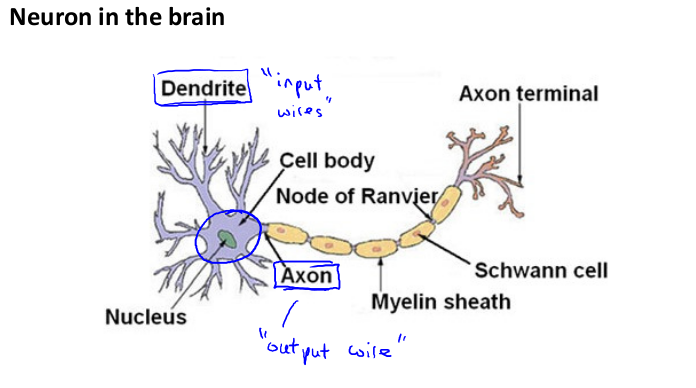
\includegraphics[width=\textwidth]{image/neuron.png}
            \caption{A biological neuron}
            \label{fig:neuron}
        \end{figure}

        Figure \ref{fig:neuron} shows a model of a biological neuron. The \textbf{dendrites} are the wires which receive input signal. The \textbf{axons} output the signal.

        \subsubsection{Neural model: logistic unit}
            In our model:
            \begin{itemize}
                \item Dendrites: input features x\textsubscript{1}, x\textsubscript{2}, \dots, x\textsubscript{n}.
                \item Output: result of hypothesis function.
                \item x\textsubscript{0}: bias unit (:= 1).
                \item Logistic function: $\frac{1}{1+exp(-\theta^T X)}$, referred to as the sigmoid(logistic) \textbf{activation} function.
                \item $\theta$ are referred to as \textbf{weights}.
            \end{itemize}

            Visually, a simplistic representation can be view as 

            \begin{equation}
                [x_0\; x_1\; x_2]\: \rightarrow \: [\:]\: \rightarrow\: h_\theta (x)
                \label{fig:visual-nn-repr}
            \end{equation}


            The input nodes (layer 1, input layer) go into the another node (layer 2), which then outputs to hypothesis function (output layer).

            In this example, we label the intermediate layers of nodes (between the input and output layers) $a^2_0, \dots, a^2_n$: \textbf{activation units}. 
            Definitions:\\

            \fbox{
                $ a_i^{(j)} $ = ``activation of unit i in layer j 
            }\\

            \fbox{
                $\Theta^{(j)}$= matrix of weights controlling function mapping from layer j to layer j+1.
            }\\
          
            If we had one hidden layer, it would look like:

            \[
                \boxed{
                [x_0 \, x_1 \, x_2\, x_3] \:\rightarrow \: [ a_1^{(2)},a_2^{(2)},a_3^{(2)}] \: \rightarrow h_\theta (x)
            }
            \]  
    
            The value for each of the activation node is obtained as follows;

            \[
                a_1^{(2)} = g (\Theta^{(1)}_{10} x_0 + \Theta^{(1)}_{11} x_1 + \Theta^{(1)}_{12} x_2+\Theta^{(1)}_{13} x_3 )
            \] 

            \[
                a_2^{(2)} = g (\Theta^{(1)}_{20} x_0 + \Theta^{(1)}_{21} x_1 + \Theta^{(1)}_{22} x_2+\Theta^{(1)}_{23} x_3 )
            \] 

            \[
                a_3^{(2)} = g (\Theta^{(1)}_{30} x_0 + \Theta^{(1)}_{31} x_1 + \Theta^{(1)}_{32} x_2+\Theta^{(1)}_{33} x_3 )
            \] 

            \[
                h_\Theta(x) = a_1^{(3)} = g (\Theta^{(1)}_{10} a_0 + \Theta^{(1)}_{11} a_1 + \Theta^{(1)}_{12} a_2+\Theta^{(1)}_{13} a_3 )
            \] 

            Essentially, each layer j has its own \textbf{matrix of weights}, $\Theta^{(j)}$.\\
            \fbox{%
                \parbox{\textwidth}{%
                 \textbf{If network has $s_j$ units in layer j and $s_{j+1}$ units in layer j+1,
                then $\Theta^{(j)}$ will be of dimension $s_{j+1} \times (s_j +1)$.
                }
                }%
            }

            The +1 comes from the addition in $\Theta^{(j)}$ of the bias nodes, $x_0$ and $\Theta_0^{(j)}$. 
            
            In the above example, layer 2 has 3 units ( $a_1^{(2)}, a_2^{(2)},a_3^{(2)}$) and layer 1 has 3 units (not including the bias unit). Therefore the weight matrix $\Theta^{(1)}$ which maps layer 1 to layer 2 is of dimension $3\times(3+1)$. 

            Another example: if layer 1 has 2 input nodes and layer 2 has 4 activation nodes- dim ($\Theta^{(1)}$) is going to be 4x3 where $s_j=2$ and $s_{j+1}=4$, so $s_{j+1}\times (s_j +1)=4\times3$.

            \subsubsection{Forward Propagation: Vectorized Implementation}
                Define a new variable: $z_k^{(j)}$ as the parameter for for the logistic function $g(z)$ such that:
                \[
                    a_1^{(2)} = g (z_1^{(2)})
                \] 
                \[
                    a_2^{(2)} = g (z_2^{(2)})
                \] 
                \[
                    a_3^{(2)} = g (z_3^{(2)})
                \] 
              
                Therefore, for layer j=2 and unit k:
                    \[
                        z_k^{(2)} = \Theta^{(1)}_{k, 0} x_0 + \Theta^{(1)}_{k, 1} x_1+ \dots+ \Theta^{(1)}_{k, n} x_n 
                    \]                
                \begin{align*}
                x = \begin{bmatrix}
                        x_0 \\
                        x_1 \\
                        \cdots \\
                        x_n
                    \end{bmatrix} \: &
                z^{(j)} = \begin{bmatrix}
                            z_1^{(j)} \\ 
                            z_2^{(j)} \\
                            \cdots \\
                            z_n^{(j)} \\
                          \end{bmatrix}
                \end{align*}
                We can further generalize by setting $\mathbf{x} = a^{(1)}$ and re-write the equation:
                \begin{equation}
                    z^{(j)} = \Theta^{(j-1)} a^{(j-1)}
                    \label{eq:activation-logistic-z}
                \end{equation}

                Dimension check:  
                \begin{itemize}
                    \item $\Theta^{(j-1)}$ is of dimension $s_j\times (n+1)$.
                    \item a\textsuperscript{(j)} is a column vector with dimension $1\times(j+1)$.
                \end{itemize}

                Thus the logistic function is applied element-wise to \textbf{z}: 
                \begin{equation}
                    a^{(j)} = g (z^{(j)})
                    \label{eq:activation}
                \end{equation}

                We then add the bias unit $a_0^{(j)} = 1$ to the activation matrix. If we propagate forward by one layer in Equation \ref{eq:activation-logistic-z}:
                \begin{equation}
                    z^{(j+1)} = \Theta^{(j)} a^{(j)}
                    \label{eq:formal-activation-x}
                \end{equation}

                The last theta matrix $\Theta^{(j)}$ will have only one row which is multiplied by one column $a^{(j)}$ such that the result is a single scalar.Hence the final hypothesis output is:

                \begin{equation}
                    h_\theta (x) = a^{(j+1)} = g (z^{(j+1)})
                    \label{eq:neural-hypothesis}
                \end{equation}



                


    \subsection{Application - Logic Gate Synthesis}
        We can apply neural networks to predict various logic gates: AND, OR, XOR, NOR.
        The basic graph can be represented as :

        \[
        \begin{bmatrix}
             x_0 \\
             x_1 \\
             x_2
        \end{bmatrix}
        \rightarrow \:
        [\; g (z^{(2)})\;]
        \rightarrow \:
        h_\Theta (x)
        \] 
       



        \subsubsection{AND Gate}
            Let the first theta matrix be:
            \[
                \Theta^{(1)} = [\;\;-30 \;\; 20 \;\; 20 \;\;]
            \] 
          
            Table \ref{tab:AND-gate} outlines the logistic hypothesis output which represents an AND gate: output = 1 $\iff$ ( $x_1=1$ and $x_2 = 1$). The intuition here in choosing the $\Theta$ parameters is that we want the sigmoid function evaluate to be positive only when both x\textsubscript{1} and x\textsubscript{2} are logic 1. Therefore, we assign the bias unit to a large negative value, such that the result of $\Theta x$ is positive only when both the two other weights are added. 

            \begin{table}
                \begin{center}
                    \begin{tabular}[htbp]{|c|c||c|c|}
                        \hline
                        $x_1$ & $x_2$ & z & $h_\Theta (x) = g(z)$ \\
                        \hline
                        \hline
                        0   &   0   &   -30     &   0\\
                        0   &   1   &   -10     &   0\\
                        1   &   0   &   -10     &   0\\
                        1   &   1   &    10     &   1\\
                        \hline
                    \end{tabular}
                \end{center}
                \caption{Truth table of AND gate}
                \label{tab:AND-gate}
            \end{table}


        \subsubsection{OR Gate}

        Similarly, Table \ref{tab:OR-gate} outlines the truth table for the OR function. We pick a parameter matrix:
            \[
                \Theta^{(1)} = [\;\;-10 \;\; 20 \;\; 20 \;\;]
            \] 
          

            \begin{table}
                \begin{center}
                    \begin{tabular}[htbp]{|c|c||c|c|}
                        \hline
                        $x_1$ & $x_2$ & z & $h_\Theta (x) = g(z)$ \\
                        \hline
                        \hline
                        0   &   0   &   -10     &   0\\
                        0   &   1   &    10     &   1\\
                        1   &   0   &    10     &   1\\
                        1   &   1   &    30     &   1\\
                        \hline
                    \end{tabular}
                \end{center}
                \caption{Truth table of OR gate}
                \label{tab:OR-gate}
            \end{table}




        \subsubsection{NOR Gate}

        Similarly, Table \ref{tab:NOR-gate} outlines the truth table for the NOR function. We pick a parameter matrix:
            \[
                \Theta^{(1)} = [\;\;10 \;\; -20 \;\; -20 \;\;]
            \] 
          

            \begin{table}
                \begin{center}
                    \begin{tabular}[htbp]{|c|c||c|c|}
                        \hline
                        $x_1$ & $x_2$ & z & $h_\Theta (x) = g(z)$ \\
                        \hline
                        \hline
                        0   &   0   &    10     &   1\\
                        0   &   1   &   -10     &   0\\
                        1   &   0   &   -10     &   0\\
                        1   &   1   &   -30     &   0\\
                        \hline
                    \end{tabular}
                \end{center}
                \caption{Truth table of NOR gate}
                \label{tab:NOR-gate}
            \end{table}


        \subsubsection{NOT Gate}

        For an inversion, we just need a single parameter x. Table \ref{tab:NOT-gate} outlines the truth table for the NOT function. We pick a parameter matrix:
            \[
                \Theta^{(1)} = [\;\;10 \;\; -20 \;\;]
            \] 
          

            \begin{table}
                \begin{center}
                    \begin{tabular}[htbp]{|c||c|c|}
                        \hline
                        $x$ & z & $h_\Theta (x) = g(z)$ \\
                        \hline
                        \hline
                        0   &    10     &   1\\
                        1   &   -10     &   0\\
                        \hline
                    \end{tabular}
                \end{center}
                \caption{Truth table of NOT gate}
                \label{tab:NOT-gate}
            \end{table}


        \subsubsection{XNOR Gate}
        
        Now, we would like to synthesize the XNOR function (shown in Table \ref{tab:XNOR-gate}. This requires a three level neural network. We can decompose the function XNOR:
            \[
                \overline{ x_1 \oplus x_2} = x_1 x_2 + \overline{x_1}\cdot \overline{x_2}
            \] 
            
            Therefore, in the second layer we will computer the AND and NOR functions then apply OR to the two intermediate output in the third layer. 


            \[
                \Theta^{(1)} = [\;\; -30 \;\; 30 \;\; 20 \;\;]
            \]

            \[
                \Theta^{(2)} = [\;\; -10 \;\; 20 \;\; 20 \;\;]
            \]
            
            
            So:
            \[
                a^{(2)}= g(\Theta^{(1)} \cdot x)
            \]
            \[
                a^{(3)}= g(\Theta^{(2)} \cdot a^{(2)})
            \]
            \[
                h_\Theta (x)= a^{(3)} 
            \] 
   

            \begin{table}
                \begin{center}
                    \begin{tabular}[htbp]{|c|c||c|c||c|}
                        \hline
                    $x_1$   &   $x_2$   &   $a_1^{(2)}$ &   $a_2^{(2)}$ &   $h_\Theta (x)$\\
                    \hline \hline
                    0       &   0       &   0           &   1           &   1 \\
                    0       &   1       &   0           &   0           &   0 \\
                    1       &   0       &   0           &   0           &   0 \\
                    1       &   1       &   1           &   0           &   1 \\
                    \hline
                    \end{tabular}
                \end{center}
                \caption{Truth table of XNOR}
                \label{tab:XNOR-gate}
            \end{table}










            \subsection{Multi-class Classification}
                For multi-class classification, our prediction will be a column vector with each element be of ``whether the current item belongs to the class of that position''. For example, for a 4-class classification, an example output would be:
                \[
                    h_\Theta (x) = [0010]
                \] 
